\Needspace{3.5in}
\begin{prob}

    Suppose a depth first search (DFS) is run on the graph below, starting at node $a$.
    Start and finish times are calculated using the convention that the start time of node $a$ is 1.

    \begin{center}
        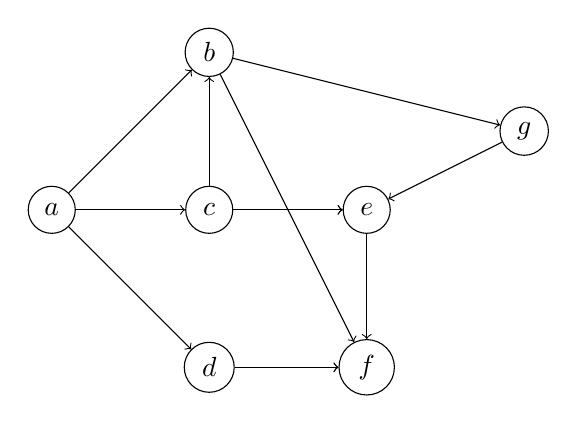
\begin{tikzpicture}
            {
                \tikzset{every node/.style = {shape=circle, draw, minimum size=17pt}}

                \node (a) at (0, 0) {$a$};
                \node (b) at (2, 2) {$b$};
                \node (c) at (2, 0) {$c$};
                \node (d) at (2, -2) {$d$};
                \node (e) at (4, 0) {$e$};
                \node (f) at (4, -2) {$f$};
                \node (g) at (6, 1) {$g$};
            }

            
            \draw (a) edge[->]  (b);
            \draw (a) edge[->]  (c);
            \draw (a) edge[->]  (d);
            \draw (b) edge[->]  (f);
            \draw (b) edge[->]  (g);
            \draw (c) edge[->]  (b);
            \draw (c) edge[->]  (e);
            \draw (d) edge[->]  (f);
            \draw (c) edge[->]  (e);
            \draw (g) edge[->]  (e);
            \draw (d) edge[->]  (f);
            \draw (e) edge[->]  (f);

        \end{tikzpicture}
    \end{center}

    What will be the \textbf{finish} time of node $c$? Assume the convention that a
    node's neighbors are produced in alphabetical order.

    \inlineresponsebox[.75in]{11}

\end{prob}
